\documentclass{iopjournal}
\usepackage{amsmath,amssymb,amsfonts}%
\usepackage{amsthm}%
\usepackage{mathrsfs}%
\usepackage{booktabs}%
\usepackage{xcolor}%
\usepackage{listings}%
\usepackage{wasysym}%
\usepackage{textcomp}%
\usepackage{manyfoot}%
\usepackage[title]{appendix}%
\usepackage{algorithm}%
\usepackage{algorithmicx}%
\usepackage{algpseudocode}%
\usepackage{enumitem}%
\usepackage[
    backend=biber,
    style=numeric,
]{biblatex}%
\addbibresource{./citations.bib}

% Options
	% [anonymous]	Provides output without author names, affiliations or acknowledgments to facilitate double-anonymous peer-review

\begin{document}

\articletype{Paper}%	 e.g. Paper, Letter, Topical Review...

\title{Absolute Time in Higher-Dimensional Geometry: Classically Simultaneous Relativity via an Unwrapped Kaluza-Klein Dimension}

\author{Andrew Mueller$^1$\orcid{0000-0003-0573-6327}}

\affil{$^1$Independent Researcher, Milwaukee, USA}

\email{AndrewMueller414@gmail.com}

\keywords{gravitation, time, relativity, Kaluza--Klein theory, Painlev\'e--Gullstrand coordinates, preferred frame}

\begin{abstract}
Special relativity is normally written with time as a fourth dimension. We show that its kinematics can instead be written with a fourth spatial axis and no time dimension. Space is given a non-compact density axis $y$, as in an unwrapped Kaluza--Klein construction, and motion along the four resulting axes is taken as the fundamental rate of change. The inclination of a body's path carries the kinematics: its slope is $\partial_x y=\beta\gamma$, its sine is the speed, and its cosine is the rate of a clock carried along it. Time is a ratio of distances along the path, light enters only as the spread of a causal sphere from each event, and every inertial observer can recover one absolute time. Gravity shares this geometry. If space flows outward from every mass, as in the Hubble flow, the space around a mass is inclined into $y$ exactly as a moving path is, and for steady fields time can be removed altogether, reproducing known orbits, light bending and perihelion advance. Where developed, the construction is equivalent to special and general relativity, so these are consistency checks rather than predictions; we identify where differences could arise.
\end{abstract}

\section{Introduction}\label{sec1}

In special relativity time is a fourth dimension of spacetime, and its rate is tied to the speed of light. Time does two jobs there: it locates events, as a fourth coordinate does, and it orders change, as a rate does. This paper keeps both jobs and removes time as a dimension. The fourth coordinate becomes a spatial one, a density axis $y$ that extends ordinary space $\mathbb{R}^3$ in the manner of an unwrapped, non-compact Kaluza--Klein dimension~\cite{Kaluza1921, Klein1926}. The rate of change becomes motion, which is primitive and is not measured against anything else. A body moves along four axes: the three of $\mathbb{R}^3$ and the density axis, along which it is carried by its own motion.

One geometric object carries the argument: the inclination of a path through $\mathbb{R}^3\times y$. Section~\ref{sec_motion} shows that it contains the kinematics of special relativity (SR)~\cite{einstein1905electrodynamics}. Its slope is $\partial_x y=\beta\gamma$, so that $\gamma=\sqrt{1+(\partial_x y)^2}$; its sine is the speed; and its cosine is the coordinate density, which is also the rate of a clock carried along the path. Time readings are ratios of distances along the path, and the speed of light enters only as the speed of the causal sphere that spreads from each event. Every inertial observer can then recover one absolute time, and the relativity of simultaneity becomes a displacement along $y$.

Section~\ref{sec_gravity} shows that gravity has the same geometry. Einstein's cosmological model of 1917 was static~\cite{Einstein1917CosmologicalConsiderations, ORaifeartaigh2017EinsteinCosmology, Nussbaumer2014EinsteinStaticToExpanding}. Here space is taken to flow outward, around every mass as in the Hubble flow. In that flow the space around a mass is inclined into $y$ exactly as a moving path is: the inclination gives the static clock rate, and the height of the inclined space is the offset between absolute and static clocks. One relation, $\beta^2=2Gm/(c^2R)$, describes the flow around a mass and the Hubble flow, and for steady fields the time coordinate can be removed from the motion of light and matter altogether. Section~\ref{sec_kk} places the density axis in a five-dimensional Kaluza--Klein metric and identifies the condition its scalar sector must meet. Section~\ref{sec_discussion} states what has been shown, how it relates to other formulations, and where it could differ from general relativity.

The construction joins several established lines of work. Mansouri and Sexl showed that absolute simultaneity is compatible with the predictions of SR~\cite{MansouriSexl1977}, and the neo-Lorentzian tradition treats relativistic effects as properties of motion relative to a preferred frame~\cite{Bell1976,Brown2005}. Euclidean relativity~\cite{Montanus2001,Almeida2001} also uses a positive-definite four-dimensional geometry. Induced-matter theory uses a non-compact fifth dimension~\cite{Wesson1999STM,OverduinWesson1997}, and the Campbell--Magaard theorem allows any analytic solution of the Einstein equations to be embedded locally in five dimensions~\cite{Campbell1926Course,Magaard1963}. The outward flow is the time reverse of the river model of black holes~\cite{HamiltonLisle2008}, and the view that time is abstracted from change is that of ephemeris time~\cite{Barbour2009}. What this paper adds is the identification of the Lorentz factor, the speed, the clock rate and the synchronization offset with one inclination in $\mathbb{R}^3\times y$, in SR and in gravity alike.

The construction is a reformulation. Where it has been developed it is equivalent to SR and to general relativity, and its gravitational results use field equations imported from general relativity, so they are consistency checks rather than predictions. Its content is the account of time it gives, and the places where an independent dynamics for $y$ could make it differ.

\begin{figure}[h]
\centering
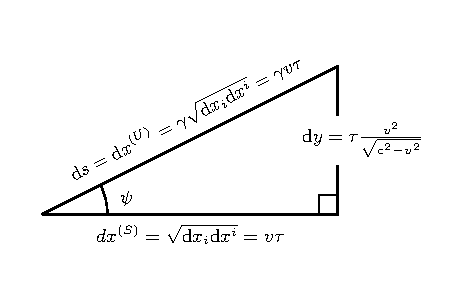
\includegraphics[width=0.75\textwidth]{../diagrams/outputs/simple_triangle.eps}
\caption{A path element through $\mathbb{R}^3\times y$: the advance $dx$ through $\mathbb{R}^3$, the advance $dy$ along the density axis, and the path length $ds=dx^{(U)}=\gamma\,dx$. The inclination $\psi$ of the path satisfies $\tan\psi=\partial_x y=\beta\gamma$ (subsection~\ref{sec_paths}).}
\label{fig_trig_diagram}
\end{figure}

\subsection{The Lighthouse \& The Clock-Tower}\label{sec_lighthouse}

The picture can be stated as a thought experiment. Let $\mathbf{S}$ be the absolute frame, and let two observers, $A$ and $B$, agree that $B$ will travel at an agreed speed $v$ relative to $\mathbf{S}$ between two points $p_1$ and $p_2$ at rest in $\mathbf{S}$, a distance $d$ apart. $A$ remains at $p_1$. At $p_2$ stands a clock tower large enough to be read from $p_1$. Its face is read by the light it sends out: a lighthouse, whose light spreads from each event as a sphere of radius $c\,\Delta t$.

We make two assertions.

\begin{enumerate}[label=\arabic*.]
\item To keep a classical simultaneity in $\mathbb{R}^{3}$, $A$ and $B$ must agree on the time at which $B$ reaches $p_{2}$.
\item To agree with the measured dilation of moving clocks~\cite{Rossi1941, FrischSmith1963, Bailey1977, Bailey1979, Botermann2014}, the clock carried by $B$ must advance by $d/(\gamma v)$ on the trip.
\end{enumerate}

Both hold if the motion of $B$ is a path through $\mathbb{R}^3\times y$ (subsection~\ref{sec_paths}). Along it $B$ advances $d$ through $\mathbb{R}^3$ and $\beta\gamma d$ along $y$, so the path has length $\gamma d$. The absolute time of the trip,

\begin{equation}\label{eq_lighthouse_time}
    \Delta\tau=\frac{d}{v}=\frac{\gamma d}{\gamma v},
\end{equation}

is the same whether it is formed from the absolute distance and speed, as $A$ does, or from the path length and the rate $\gamma v$ along the path, as $B$ does. In the second form the speed is divided by the coordinate density $1/\gamma$: a speed referred to the path dilates inversely with the coordinate density. The clock of $B$ reads $d/(\gamma v)$ (subsection~\ref{sec_paths}), which satisfies the second assertion. The light from the clock tower does not define the time of the trip; it is how the time is read. Because every reading is carried by light, time appears to pass at $c$. A photon is the limit of the construction in which the path turns entirely along $y$ and the coordinate density vanishes (subsection~\ref{sec_paths}).

\section{Motion without Time}\label{sec_motion}

This section builds the kinematics of SR from the two properties of time that the model keeps: a fourth displacement coordinate, the position along $y$, and a driving rate of change, motion. Throughout, $\mathbf{S}$ is the absolute frame in which $\mathbb{R}^3$ is at rest, and $\tau$ is its time. $\tau$ is not an independent coordinate: subsection~\ref{sec_paths} obtains $c\tau$ as a ratio of lengths along a path, so seconds enter only through the value of $c$. We also require that, in a frame co-moving along $y$, mechanical equations reduce to their Newtonian forms, with only the relativistic part of each magnitude extending along $y$. Table~\ref{table_dictionary} lists the quantities used and their standard counterparts.

\begin{table}[h]
\caption{Quantities of this paper and their standard counterparts}%
\label{table_dictionary}
\begin{tabular}{@{}p{0.40\linewidth}p{0.54\linewidth}@{}}
\toprule
This paper & Standard counterpart\\
\midrule
$\psi$, $\tan\psi=\partial_x y$ & inclination of a path, or of the Flamm surface, in $\mathbb{R}^3\times y$; $\psi=\mathrm{gd}(\eta)$, the Gudermannian of the rapidity\\
$\sin\psi=\beta=v/c$ & speed; in gravity the flow velocity, which is the shift vector (``river velocity'') and the escape velocity from the enclosed mass\\
$\cos\psi=1/\gamma$ & coordinate density; the rate of a moving clock, and the static lapse in the exterior vacuum region, but not generally inside matter\\
$c\,d\tau=dx\,ds/dy$, $c\,dt_U=dx^2/dy$ & absolute time and proper time of a moving clock\\
$y(R)$, $\partial_R y=\beta\gamma$ & Flamm embedding of the static slice, $d\ell^2=dR^2+dy^2$\\
$\partial_\tau y=v^2/\sqrt{c^2-v^2}$ & $dy/dT$ along a worldline at rest in the outward flow\\
$\delta(M,R)=2GM/R^3$ & radial tidal eigenvalue\\
\bottomrule
\end{tabular}
\end{table}

\subsection{The Fourth Coordinate and the Lorentz Factor}\label{sec_fourth_coordinate}

Let a body move at speed $v$ relative to $\mathbf{S}$, and let the additional coordinate grow along its motion as

\begin{equation}\label{eq_dy_definition}
    y=\tau\frac{v^2}{\sqrt{c^2-v^2}} .
\end{equation}

With $x=v\tau$ this gives

\begin{equation}\label{eq_dy_dtau}
    \partial_\tau y=\frac{v^2}{\sqrt{c^2-v^2}}=\frac{\gamma v^2}{c},
\end{equation}

\begin{equation}\label{eq_dy_dx}
    \partial_x y=\frac{v}{\sqrt{c^2-v^2}}=\beta\gamma ,
\end{equation}

and $v\,\partial_x y=\partial_\tau y$. Squaring equation~\eqref{eq_dy_dx} and using $\gamma^2=1/(1-\beta^2)$ gives

\begin{equation}\label{eq_gamma_dy_dx}
    \gamma=\sqrt{1+\left(\partial_x y\right)^2},
\end{equation}

so the Lorentz factor is the slope of the additional coordinate. The length of a path element through $\mathbb{R}^3\times y$ is then

\begin{equation}\label{eq_path_length}
    ds^2=dx^2+dy^2=\gamma^2dx^2 .
\end{equation}

This is the separation $dx'=\gamma\,dx$ that the Lorentz transformation assigns, in the frame $\mathbf{U}$ moving at $v$, to two events separated by $dx$ at equal $\tau$. The same transformation gives $c\,dt'=-\gamma(v/c)\,dx=-dy$ for these events, and the interval is preserved, $c^2dt'^2-dx'^2=dy^2-\gamma^2dx^2=-dx^2$. Subsection~\ref{sec_classical_simultaneity} extends this from equal-$\tau$ separations to arbitrary events. The relation to the rapidity $\eta$ is elementary: $\gamma=\cosh\eta$ and $\partial_x y=\sinh\eta$, so equation~\eqref{eq_gamma_dy_dx} is the identity $\cosh^2\eta=1+\sinh^2\eta$.

\subsection{Motion as Paths through \texorpdfstring{$\mathbb{R}^3\times y$}{R3 x y}}\label{sec_paths}

A motion is a path through $\mathbb{R}^3\times y$. It carries no time parameter; its only property at each point is its direction. Let $\psi$ be the inclination of the path above $\mathbb{R}^3$ (figure~\ref{fig_trig_diagram}). Equation~\eqref{eq_dy_dx} gives $\tan\psi=\partial_x y=\beta\gamma$, and hence

\begin{equation}\label{eq_path_angle}
    \sin\psi=\frac{dy}{ds}=\beta,
    \qquad
    \cos\psi=\frac{dx}{ds}=\frac{1}{\gamma}.
\end{equation}

The two direction cosines are the rates of the model. The speed is the advance along $y$ per unit path, $\sin\psi$: a body is propelled along the density axis by its motion, and its speed is that propulsion. The fraction $\cos\psi$ of the path that lies in $\mathbb{R}^3$ is the coordinate density, the number of absolute coordinates per measured length, and it is also the rate of a clock carried along the path.

\paragraph{Time readings as ratios of distances.} Along a path element with advances $dx$ and $dy$, the absolute time and the reading of a clock carried along the path are

\begin{equation}\label{eq_path_times}
    c\,d\tau=\frac{dx\,ds}{dy}=\frac{dx}{\sin\psi},
    \qquad
    c\,dt_U=\frac{dx^2}{dy}=\frac{dx}{\tan\psi}.
\end{equation}

They give $dx=v\,d\tau$, the moving-clock rate $dt_U=d\tau/\gamma$, and $c\,dt_U=\gamma c\,d\tau-dy$ along the path, which are items 4 and 1 of the Proposition in subsection~\ref{sec_classical_simultaneity}. Neither reading is an independent coordinate. Both are lengths formed from the path.

\paragraph{The causal sphere.} Light spreads from each event as a sphere of radius $c\,d\tau$. While a body advances $dx$ through $\mathbb{R}^3$ the sphere reaches $c\,d\tau=dx/\sin\psi$, so

\begin{equation}\label{eq_causal_sphere}
    \frac{dx}{c\,d\tau}=\sin\psi\leq1 ,
\end{equation}

and every body remains inside the causal sphere of its own past events. This is the only place where $c$ enters. The path itself does not advance at $c$: its length per unit of light distance, $ds/(c\,d\tau)=\beta\gamma=\tan\psi$, takes any value. Time is read off the causal sphere, so it appears to pass at $c$; the rate of change that the model identifies with time is the motion along the four axes, which is not bound to that rate. Whether the two rates can be told apart by measurement is discussed in subsection~\ref{sec_two_rates}.

\paragraph{Composition.} With $\tanh\eta=\beta$, the inclination is the Gudermannian of the rapidity, $\psi=\mathrm{gd}(\eta)=\arctan(\sinh\eta)$. Collinear motions compose by adding rapidities, so $\sin\psi_W=\tanh(\eta_1+\eta_2)=(\beta_1+\beta_2)/(1+\beta_1\beta_2)$, the relativistic composition of velocities.

\paragraph{Limits.} A body at rest has no path ($dx=dy=0$), and equation~\eqref{eq_path_times} gives it no time reading of its own. Its time must come from other change: its internal motion, or the motion of everything else, as in ephemeris time~\cite{Barbour2009}. Light is the limit $\psi\to90^\circ$, in which the coordinate density $\cos\psi$ vanishes, the clock reading $c\,dt_U$ goes to zero, and $c\,d\tau$ goes to $dx$, the radius of the causal sphere. The limit is consistent but degenerate.

\paragraph{Relation to Euclidean relativity.} Euclidean relativity~\cite{Montanus2001,Almeida2001} writes $(c\,d\tau)^2=dx^2+(c\,d\tau_p)^2$, with the proper time $\tau_p$ as a fourth spatial coordinate, and postulates that everything moves through that space at $c$. Its worldline makes the angle $\psi$ with the proper-time axis, $\tan\psi=dx/(c\,d\tau_p)=\beta\gamma$. The path triangle $(dx,dy;ds)$ of this paper is therefore similar to its triangle $(c\,d\tau_p,dx;c\,d\tau)$, scaled by $\tan\psi$. The postulate is not used here, and the constructions differ: the path of this paper advances at $ds/(c\,d\tau)=\tan\psi$, not at $c$.

The next subsection uses these readings to show that every inertial observer recovers the same absolute time.

\subsection{Classical Simultaneity in \texorpdfstring{$\mathbb{R}^3$}{R3}}\label{sec_classical_simultaneity}

Subsection~\ref{sec_fourth_coordinate} treated two events at equal $\tau$. Here, once the displacement along $y$ is included, every inertial observer assigns the same absolute time $\tau$ to every event, and the relativity of simultaneity is entirely a displacement along $y$.

Let events be labelled by an absolute position $x$ in $\mathbb{R}^3$ (one axis is shown) and by the absolute time $\tau$, both referred to the frame $\mathbf{S}$. An observer $\mathbf{U}$ moving at velocity $v$ relative to $\mathbf{S}$ assigns to each event the displacement

\begin{equation}\label{eq_y_offset}
    y_U(x)=\gamma\frac{v}{c}\,x ,
\end{equation}

which is equation~\eqref{eq_dy_dx} integrated at fixed velocity.

\paragraph{Proposition.} For every event $(x,\tau)$ and every inertial observer $\mathbf{U}$ moving at $v$ relative to $\mathbf{S}$:
\begin{enumerate}
\item the Lorentz coordinates of $\mathbf{U}$ are
\begin{equation}\label{eq_observer_clock}
    x_U=\gamma\left(x-v\tau\right),
    \qquad
    c\,t_U=\gamma c\,\tau-y_U(x) ;
\end{equation}
\item every observer recovers the same absolute time,
\begin{equation}\label{eq_tau_recovered}
    \tau=\frac{c\,t_U+y_U(x)}{\gamma c} ;
\end{equation}
\item two events with $\Delta\tau=0$ and any separation $\Delta x$ satisfy $c\,\Delta t_U=-\Delta y_U$;
\item along the worldline of $\mathbf{U}$, $x=v\tau$, the clock of $\mathbf{U}$ advances by $dt_U=d\tau/\gamma$;
\item for an observer $\mathbf{W}$ moving at $v_2$ relative to $\mathbf{U}$, items 1 to 4 hold with $v$ replaced by the velocity of $\mathbf{W}$ relative to $\mathbf{S}$, $v_W=(v+v_2)/(1+vv_2/c^2)$.
\end{enumerate}

\begin{proof}
1. With $\tau$ as the time coordinate of $\mathbf{S}$, the Lorentz transformation gives $x_U=\gamma(x-v\tau)$ and
\begin{equation}
    c\,t_U=\gamma\left(c\tau-\frac{v}{c}x\right)=\gamma c\,\tau-\gamma\frac{v}{c}x=\gamma c\,\tau-y_U(x),
\end{equation}
using equation~\eqref{eq_y_offset}.

2. Solving equation~\eqref{eq_observer_clock} for $\tau$ gives equation~\eqref{eq_tau_recovered}. The right-hand side uses only quantities assigned by $\mathbf{U}$ and its velocity relative to $\mathbf{S}$, and it returns the same $\tau$ for every $v$.

3. Subtracting equation~\eqref{eq_observer_clock} for two events at equal $\tau$ gives $c\,\Delta t_U=-\gamma(v/c)\Delta x=-\Delta y_U$.

4. On $x=v\tau$, $y_U=\gamma v^2\tau/c$, so
\begin{equation}
    c\,t_U=\gamma c\,\tau\left(1-\frac{v^2}{c^2}\right)=\frac{c\,\tau}{\gamma}.
\end{equation}
The clock of $\mathbf{U}$ loses, relative to $\gamma c\,d\tau$, exactly its own advance $dy_U=\gamma(v/c)\,v\,d\tau$ along $y$.

5. Collinear boosts compose by addition of rapidities, so the boost at $v$ followed by the boost at $v_2$ is the boost at $v_W$ with $\gamma_W=\gamma\gamma_2(1+vv_2/c^2)$. Items 1 to 4 then follow with $v_W$ and $y_W(x)=\gamma_W(v_W/c)\,x$.
\end{proof}

The conventional time difference $\Delta t_U=-\gamma v\Delta x/c^2$ between two events at the same $\tau$ is therefore not a difference in absolute time. It is the displacement $\Delta y_U$ that $\mathbf{U}$ assigns to their separation, and all of $\mathbb{R}^3$ at a given $\tau$ is one instant for every observer. Item 4 obtains the slowing of a moving clock from its displacement along $y$; it does not insert time dilation separately. In the language of subsection~\ref{sec_paths}, the clock rate $1/\gamma$ is the coordinate density $\cos\psi$ of the path. For $\Delta\tau=0$ the absolute separation is the same for every observer, $\Delta x^2=\Delta x_U^2-(c\Delta t_U)^2=\Delta x_U^2-\Delta y_U^2$. This is the embedding relation $\Delta x_U^2=\Delta x^2+\Delta y_U^2$ read with the absolute length as the invariant. The separation $\Delta x_U$ measured by $\mathbf{U}$ is the hypotenuse of the graph of $y_U$ over $\mathbb{R}^3$ and depends on the observer, while its projection $\Delta x$ onto $\mathbb{R}^3$ does not. With $w=c\tau$, a length, item~1 reads $x_U=\gamma\left(x-\beta w\right)$ and $w_U=c\,t_U=\gamma w-y_U$. The transformation acts on lengths alone, and its invariant, $x_U^2-w_U^2=x^2-w^2$, is the Minkowski interval written in them; the geometry of subsection~\ref{sec_paths} reads the same transformation as the inclination of a path.

The frame $\mathbf{S}$ is an assumption of the model. Nothing in the kinematics singles it out, and every local experiment gives the same result in it as in any other inertial frame. We identify it with the frame of the flow of space: the cosmic rest frame on large scales, whose velocity relative to an observer is measured by the dipole of the cosmic microwave background, and the outward flow of section~\ref{sec_gravity} near a mass. The next section shows that the same inclination, and the same offset along $y$, appear in gravity.

\section{Gravity as Inclined Space}\label{sec_gravity}

In SR the inclination of a path is set by the speed of the body. In gravity it is set by the flow of space. This section takes the flow first. It then shows that the space around a mass is inclined into $y$ by the flow speed, that the inclination fixes the clock rate, that one constraint governs the flow around a mass and the expansion of the universe, and that for steady flows time can be removed from the motion of light and matter.

\subsection{The Outward Flow}\label{sec_pg_relation}

With $\beta^2=r_s/R$ the Schwarzschild metric can be written in the Painlev\'e--Gullstrand form~\cite{Painleve1921,Gullstrand1922,MartelPoisson2001}

\begin{equation}\label{eq_pg_metric}
    ds^2=-c^2dT^2+\left(dR-\beta c\,dT\right)^2+R^2d\Omega^2 ,
\end{equation}

where $T$ is the proper time of observers that move radially outward at exactly the escape velocity $\beta c$. The surfaces $T=\text{const}$ are intrinsically flat. We take these observers to be at rest in absolute space. Space then flows radially outward from the mass, in the same direction as the Hubble flow, and an observer held at fixed $R$ moves inward relative to space at $u=-\beta c$. At the surface of the Earth space streams outward at the escape velocity, about $11.2~\mathrm{km\,s^{-1}}$, while the radius of the Earth does not change. The outward direction is a postulate of the model. Both directions describe the same spacetime outside a horizon, and the inward form is the river model~\cite{HamiltonLisle2008}. Inside $r_s$ the outward form covers the time reverse of a black-hole interior, not the interior of a black hole formed by collapse, so the results here concern exteriors and ordinary stars.

The Hubble flow has the same form. For flat FLRW, $R=a(t)r$ gives $a\,dr=dR-HR\,dt$ and

\begin{equation}\label{eq_flrw_pg}
    ds^2=-c^2dt^2+\left(dR-\beta_H c\,dt\right)^2+R^2d\Omega^2,
    \qquad
    \beta_H=\frac{HR}{c}
\end{equation}

with a shift of the same, outward sign. For constant $H$ the two flows combine into one, $\beta^2=r_s/R+H^2R^2/c^2$, whose static form is the Schwarzschild--de Sitter metric; how the flows of nested systems combine in general is not established. With $m=\tfrac{4\pi}{3}\rho R^3$ and the Friedmann equation $H^2=8\pi G\rho/3$, the Hubble flow obeys $\beta_H^2=2Gm/(c^2R)$. The Hubble radius $c/H$, where $\beta=1$, is the apparent horizon of flat FLRW~\cite{Faraoni2011,Faraoni2022}, and its Newtonian counterpart is the zero-energy condition of Milne and McCrea~\cite{Milne1934,McCreaMilne1934}. More generally, marginally bound pressureless dust (the Lema\^itre--Tolman--Bondi solutions~\cite{Lemaitre1933,Tolman1934,Bondi1947} with zero energy function) takes the form~\eqref{eq_pg_metric} with $\beta^2=2Gm(R,T)/(c^2R)$ and $m$ the Misner--Sharp mass~\cite{MisnerSharp1964}, and the generalized form extends to pressure~\cite{LaskyLun2006}. Binding and expansion are one outward flow, with different distributions of mass (table~\ref{table_pg_cases}).

\begin{table}[h]
\caption{Cases of $\beta^2=2Gm/(c^2R)$ with unit lapse and flat slices}%
\label{table_pg_cases}
\begin{tabular*}{\linewidth}{@{\extracolsep{\fill}} l l l l }
\toprule
Configuration & $m(R)$ & Flow & Static-slice embedding\\
\midrule
Exterior of a mass& $M$ & outward & paraboloid\\
Uniform density ball& $\tfrac{4\pi}{3}\rho R^3$ & outward & cap of a $3$-sphere, $L^2=3c^2/8\pi G\rho$\\
Critical density (flat FLRW)& $\tfrac{4\pi}{3}\rho_c R^3$ & outward & none (de Sitter: cap, $L=c/H$)\\
\bottomrule
\end{tabular*}
\end{table}

\subsection{The Inclined Space around a Mass}\label{sec_inclined_space}

The rest space of an observer held at fixed $R$ has the radial component

\begin{equation}\label{eq_rest_space}
    h_{RR}=g_{RR}-\frac{g_{TR}^2}{g_{TT}}=1+\beta^2\gamma^2=\gamma^2,
    \qquad
    \gamma=\frac{1}{\sqrt{1-\beta^2}},
\end{equation}

so its proper radial length is $d\ell=\gamma\,dR$, and $\gamma$ is the Lorentz factor of the flow relative to that observer. This is the path relation~\eqref{eq_path_length} with $x$ replaced by the radius $R$ of the flat slice. The static slice is the graph of a height $y(R)$ over the flat slice,

\begin{equation}\label{eq_flamm_slope}
    \partial_R y=\beta\gamma,
    \qquad
    d\ell^2=dR^2+dy^2 ,
\end{equation}

which is the Flamm embedding~\cite{Flamm1916} of the Schwarzschild spatial slice, $y=\pm2\sqrt{r_s(R-r_s)}+C$. The space around a mass is therefore inclined into $y$ exactly as a path is (figure~\ref{fig_trig_diagram}), with the flow speed in place of the speed of the body:

\begin{equation}\label{eq_flamm_angle}
    \sin\psi=\beta,
    \qquad
    \cos\psi=\frac{1}{\gamma}=\frac{dR}{d\ell}.
\end{equation}

\paragraph{The height is the synchronization offset.} The change of time $dT=dt-\beta\,dR/\left[c(1-\beta^2)\right]$ takes the flow form~\eqref{eq_pg_metric} to the static form

\begin{equation}\label{eq_static_form}
    ds^2=-(1-\beta^2)\,c^2dt^2+\frac{dR^2}{1-\beta^2}+R^2d\Omega^2 ,
\end{equation}

and the offset between the absolute time $T$ and the static time $t$ is

\begin{equation}\label{eq_sync_gap_flamm}
    c\left(dT-dt\right)=-\frac{\beta}{1-\beta^2}\,dR=-\gamma\left(\beta\gamma\,dR\right)=-\gamma\,dy ,
\end{equation}

In the proper time of the static observer, $N\,c\,(dT-dt)=-dy$ with $N=1/\gamma$: the offset is the height itself. The static observer moves inward relative to space at $u=-\beta c$, so light it sends outward travels with the flow at $c(1+\beta)$ and returns against it at $c(1-\beta)$. Its synchronization parameter is $\epsilon=(1-\beta)/2$~\cite{Reichenbach1958}, the value $\tfrac12(1+u/c)$ of an observer moving at $u$, and $dy=(1-2\epsilon)\,d\ell$. The structure is that of item~3 of the Proposition: the flat slice supplies the observer-independent base $dR$, the static proper length $\gamma\,dR$ is the arc length of the graph, and a separation along $y$ is a difference in clock setting at one absolute time.

\paragraph{The inclination is fixed by the enclosed mass.} A hypersurface $y(x)$ of flat $\mathbb{R}^4$ has extrinsic curvature $K_{ij}=\partial_i\partial_j y/\sqrt{1+|\nabla y|^2}$, and its intrinsic curvature follows from the Gauss equation, ${}^{(3)}\!R=K^2-K_{ij}K^{ij}$. For a spherical profile,

\begin{equation}\label{eq_gauss_radial}
    {}^{(3)}\!R=\frac{2}{R^2}\frac{d}{dR}\left(R\,\beta^2\right)
\end{equation}

Imposing the time-symmetric Hamiltonian constraint of general relativity, ${}^{(3)}\!R=16\pi G\rho/c^2$, and integrating from a regular centre gives

\begin{equation}\label{eq_beta_enclosed}
    \beta^2(R)=\frac{2G\,m(R)}{c^2R},
    \qquad
    m(R)=\int_0^R4\pi\rho R'^2\,dR'
\end{equation}

so $\beta c$ is the escape velocity from the enclosed mass. The constraint is imported from general relativity. What the embedding adds is its expression through the Hessian of $y$, which ties the mass density to the curvature of the inclined space. Outside a mass the profile is the paraboloid above. A ball of uniform density gives $\beta^2=R^2/L^2$ with $L^2=3c^2/(8\pi G\rho)$ and $y=\pm\sqrt{L^2-R^2}+C$, a cap of a three-sphere of radius $L$, which is the spatial geometry of the interior Schwarzschild solution. The constraint used here holds on a static slice, which the Hubble flow does not have; for the Hubble flow the same relation holds on its flat slices through the constraint of subsection~\ref{sec_coordinate_density}.

\subsection{The Clock Rate}\label{sec_lapse_derivation}

The inclined space fixes the spatial geometry but not the clock rate. The embedded slice carries no information about $g_{00}$, and the Schwarzschild spacetime cannot be embedded as a hypersurface of five-dimensional flat space: it is of embedding class two, with a flat embedding known only in six dimensions~\cite{Kasner1921}. In a static vacuum region the clock rate nevertheless follows from the inclination once the second static field equation is imposed. The only imported input is the static vacuum Einstein system; the lapse itself is not assumed.

\paragraph{Static vacuum equations in embedding form.}
We write the static metric as $ds^2=-N^2c^2dt^2+h_{ij}dx^idx^j$, with $h_{ij}$ the metric induced on the embedded slice. The vacuum Einstein equations reduce to

\begin{equation}\label{eq_static_vacuum}
    {}^{(3)}\!R_{ij}=\frac{1}{N}\nabla_i\nabla_jN,
    \qquad
    \Delta N=0
\end{equation}

The trace of the first equation is ${}^{(3)}\!R=\Delta N/N$, so together they imply the time-symmetric Hamiltonian constraint ${}^{(3)}\!R=0$ already used in equation~\eqref{eq_beta_enclosed}. For a hypersurface of flat $\mathbb{R}^4$ the Gauss equation gives ${}^{(3)}\!R_{ijkl}=K_{ik}K_{jl}-K_{il}K_{jk}$, hence ${}^{(3)}\!R_{ij}=K\,K_{ij}-K_{ik}K^{k}{}_{j}$. The first equation of~\eqref{eq_static_vacuum} becomes

\begin{equation}\label{eq_lapse_hessian}
    \nabla_i\nabla_jN=N\left(K\,K_{ij}-K_{ik}K^{k}{}_{j}\right),
    \qquad
    K_{ij}=\frac{\partial_i\partial_jy}{\sqrt{1+|\nabla y|^2}}
\end{equation}

The Hessian of the lapse is fixed by the Hessian of the fourth coordinate. Equation~\eqref{eq_lapse_hessian} is a linear equation for $N$ once $y$ is known.

\paragraph{Curvatures of the radial slice.}
For a spherical profile $y(R)$ with $\partial_Ry=\beta\gamma$, the tangent plane of the embedded slice is tilted from the $R$-axis by the inclination $\psi$ of equation~\eqref{eq_flamm_angle}, and $d\ell=\gamma\,dR$ is the proper radial length. The principal curvatures are the rates at which the tilt changes along each direction:

\begin{equation}\label{eq_principal_curvatures}
    \kappa_\theta=\kappa_\phi=\frac{\sin\psi}{R}=\frac{\beta}{R},
    \qquad
    \kappa_R=\frac{d\psi}{d\ell}=\frac{d\psi}{dR}\frac{dR}{d\ell}=\frac{\beta'}{\cos\psi}\cos\psi=\beta'
\end{equation}

The sectional curvatures are $\kappa_R\kappa_\theta=\beta\beta'/R$ and $\kappa_\theta\kappa_\phi=\beta^2/R^2$, so in an orthonormal frame

\begin{equation}
    {}^{(3)}\!R_{\hat R\hat R}=\frac{2\beta\beta'}{R},
    \qquad
    {}^{(3)}\!R_{\hat\theta\hat\theta}=\frac{\beta\beta'}{R}+\frac{\beta^2}{R^2}
\end{equation}

Their trace, ${}^{(3)}\!R={}^{(3)}\!R_{\hat R\hat R}+2\,{}^{(3)}\!R_{\hat\theta\hat\theta}=4\beta\beta'/R+2\beta^2/R^2=(2/R^2)\,d(R\beta^2)/dR$, reproduces equation~\eqref{eq_gauss_radial}, which is a check on~\eqref{eq_principal_curvatures}.

If we let the exterior slice of a static, spherically symmetric vacuum region be the embedding with $\partial_Ry=\beta\gamma$ and $\beta^2=r_s/R$, and let $N\to1$ as $R\to\infty$, then equation~\eqref{eq_lapse_hessian} implies

\begin{equation}
    N(R)=\sqrt{1-\frac{r_s}{R}}=\frac{1}{\gamma}
\end{equation}

\begin{proof}
In an orthonormal frame the angular Hessian of $N$ is $\nabla_{\hat\theta}\nabla_{\hat\theta}N=(R_{,\ell}/R)\,N_{,\ell}$ with $R_{,\ell}=1/\gamma$ and $N_{,\ell}=N'/\gamma$, that is $N'/(\gamma^2R)$. The angular component of the first equation in~\eqref{eq_static_vacuum} reads

\begin{equation}
    \frac{N'}{\gamma^2RN}=\frac{\beta\beta'}{R}+\frac{\beta^2}{R^2}
    \quad\Longrightarrow\quad
    \frac{N'}{N}=\gamma^2\left(\beta\beta'+\frac{\beta^2}{R}\right)
\end{equation}

For $\beta^2=r_s/R$ one has $\beta'=-\beta/(2R)$, so $\beta\beta'+\beta^2/R=\beta^2/(2R)$ and

\begin{equation}
    \frac{N'}{N}=\frac{\gamma^2\beta^2}{2R}=\frac{r_s}{2R^2\left(1-r_s/R\right)}=\frac12\frac{d}{dR}\ln\!\left(1-\frac{r_s}{R}\right)
\end{equation}

Integrating with $N(\infty)=1$ gives the stated result. The radial component, $N_{,\ell\ell}/N=2\beta\beta'/R$, is then satisfied identically.
\end{proof}

Consequently $g_{00}\,h_{RR}=-1$ follows in this region from the embedding and the static field equations; it is not an additional assumption. The redshift factor equals $\cos\psi$, the foreshortening of the embedded slice and the coordinate density of a path with the same inclination. The same relation is what the Painlev\'e--Gullstrand change of time in section~\ref{sec_pg_relation} produces, so the two routes agree.

With the lapse, the gravitational acceleration and the radial tidal eigenvalue are derivatives of one dimensionless potential, $\vec g=\tfrac{c^2}{2}\nabla\beta^2$ and $\delta(M,R)=\tfrac{c^2}{2}\,\partial_R^2\beta^2=2GM/R^3$. A circular orbit has the locally measured speed $v_{\mathrm{local}}^2=c^2R\,N'/N=GM/(R-r_s)$, which is $\beta^2c^2/2$ to leading order: an orbital speed is not the flow speed. The static clock rate is the cosine of the inclination of the space in which the clock sits, as the rate of a moving clock is the cosine of the inclination of its path.

\paragraph{Free fall and the role of marginal binding.}
Let $u$ be a radial geodesic with relative Lorentz factor $\gamma_{\rm rel}$ with respect to the static observers. Contracting with the Killing vector $\xi=\partial_t$ gives the conserved energy per unit mass, $E=N\gamma_{\rm rel}$. For a body released from rest at infinity, or for its time reverse, a body moving outward at exactly the escape velocity, $E=1$, hence $\gamma_{\rm rel}=1/N=\gamma$ and $\beta_{\rm rel}=\beta$, which is the identification used to define $y$. For a body released from rest at $R_0$, $E=N(R_0)$ and

\begin{equation}
    \gamma_{\rm rel}(R)=\frac{N(R_0)}{N(R)},
    \qquad
    \beta_{\rm rel}^2=1-\frac{N(R)^2}{N(R_0)^2}\neq\beta^2
\end{equation}

The slope $\beta\gamma$ of the Flamm embedding therefore coincides with $\beta_{\rm rel}\gamma_{\rm rel}$ only for the marginally bound congruence. Bound orbits are not described by a different embedding of the same slice but by a different relation between the flow and the slope. The orbit results of Appendix~\ref{app_orbits} use the static geometry and standard geodesics and are unaffected, but the reading of $y$ as ``the displacement of the flow frame'' is specific to $E=1$.

\paragraph{Matter.} The same steps extend from vacuum to a static perfect fluid with density $\rho(R)$ and pressure $p(R)$. The slice is unchanged: equation~\eqref{eq_beta_enclosed} holds for any density, so $\beta^2=2Gm(R)/(c^2R)$ and $\gamma^2=1/(1-\beta^2)$. The static Einstein equations with a fluid at rest read

\begin{equation}
    {}^{(3)}\!R_{ij}-\frac{1}{N}\nabla_i\nabla_jN=\frac{4\pi G}{c^{4}}\left(\rho c^{2}-p\right)h_{ij}
\end{equation}

The angular component, with the embedding values ${}^{(3)}\!R_{\hat\theta\hat\theta}=\beta\beta'/R+\beta^2/R^2$ and the identity $\left(R\beta^2\right)'=8\pi G\rho R^2/c^2$, gives

\begin{equation}\label{eq_interior_lapse}
    \frac{N'}{N}=\gamma^{2}\left(\frac{\beta^{2}}{2R}+\frac{4\pi G\,p\,R}{c^{4}}\right)
    =\frac{G\left(m+4\pi R^{3}p/c^{2}\right)}{c^{2}R^{2}\left(1-2Gm/c^{2}R\right)}
\end{equation}

This is the potential gradient of the Tolman--Oppenheimer--Volkoff (TOV) equation~\cite{Tolman1939,OppenheimerVolkoff1939}. The radial component is then satisfied identically provided $p'=-\left(\rho c^2+p\right)N'/N$, which is hydrostatic equilibrium. Outside the matter $p=0$ and equation~\eqref{eq_interior_lapse} reduces to the vacuum result $N=1/\gamma$. Inside matter $N\neq1/\gamma$: the pressure term adds to the redshift beyond the foreshortening of the slice.

\paragraph{Uniform density.} For $\rho=\text{const}$, $\beta^2=R^2/L^2$ with $L^2=3c^2/(8\pi G\rho)$, and the slice is the spherical cap found above. Writing $s(R)=\cos\psi=1/\gamma=\sqrt{1-R^2/L^2}$ and $s_*=s(R_*)$, equation~\eqref{eq_interior_lapse} and hydrostatic equilibrium are solved by

\begin{equation}\label{eq_uniform_interior}
    N(R)=\frac{3s_*-s(R)}{2},
    \qquad
    p(R)=\rho c^{2}\,\frac{s(R)-s_*}{3s_*-s(R)}
\end{equation}

with $N(R_*)=s_*=\sqrt{1-r_s/R_*}$ and $p(R_*)=0$, the interior Schwarzschild solution. The interior lapse is $\tfrac32\cos\psi_*-\tfrac12\cos\psi(R)$ in terms of the tilt of the slice.

\paragraph{Buchdahl bound.} The central pressure is $p_c/\rho c^2=(1-s_*)/(3s_*-1)$, which is finite only for $3s_*>1$. In terms of the slice this means $\gamma_*<3$, or $\cos\psi_*>1/3$, a tilt of the slice at the surface below $70.5^\circ$, which is the same as

\begin{equation}
    R_*>\frac{9}{8}\,r_s
\end{equation}

At the limit $N(0)=(3s_*-1)/2\to0$ and the central pressure diverges. This recovers the Buchdahl compactness limit~\cite{Buchdahl1959} for the uniform-density solution. The general Buchdahl theorem for non-increasing density profiles is not derived in this paper; the nonuniform example below is an application of the interior equations, not a proof of that theorem.

\paragraph{A nonuniform profile.} For the Tolman VII density $\rho=\rho_c\left(1-R^2/R_*^2\right)$~\cite{Tolman1939} the slice is no longer a cap. With $x=R/R_*$ and the compactness $C=2GM/(c^2R_*)$, equation~\eqref{eq_beta_enclosed} gives $\beta^2=C\left(\tfrac52x^2-\tfrac32x^4\right)$, whose maximum is $\tfrac{25}{24}C$, so the embedding is real throughout the star only for $C<\tfrac{24}{25}$. This is necessary for a regular static embedding but not sufficient for a finite central pressure. The pressure and lapse follow from equation~\eqref{eq_interior_lapse} and hydrostatic equilibrium by integration from the surface, where they match the exterior values, $p=0$ and $N=\sqrt{1-C}=1/\gamma$. As in the uniform case, this is general relativity written in the variables of the embedding, not an independent prediction.

\subsection{Coordinate Density and Its Rate of Change}\label{sec_coordinate_density}

The two properties of time that the model keeps, a fourth displacement coordinate and a rate of change, have a precise counterpart in the flow: the coordinate density, and the rate at which the flow changes it.

\paragraph{Coordinate density.} Outside a mass a static observer measures $d\ell=\gamma\,dR$ along a radial interval whose absolute length is $dR$. The number of absolute coordinates per measured length is therefore
\begin{equation}\label{eq_density_lapse}
    \frac{dR}{d\ell}=\frac{1}{\gamma}=N ,
\end{equation}
the static clock rate, and the cosine of the inclination $\psi$ of the Flamm surface, as for a path (subsection~\ref{sec_paths}). The equality holds because $g_{tt}g_{RR}=-c^2$ in the Schwarzschild exterior. In vacuum the coordinate density and the rate of time are the same quantity. Inside matter the lapse differs from $1/\gamma$ by the pressure terms of subsection~\ref{sec_lapse_derivation}, so equation~\eqref{eq_density_lapse} is a vacuum statement.

\paragraph{Rate of change.} The flow $\vec v$ of absolute space changes the coordinate density at the rate $\theta=\nabla\cdot\vec v$, the fractional rate of change of a volume element carried by the flow. The shear $\sigma_{ij}$ is the trace-free part of $\partial_{(i}v_{j)}$. With unit lapse and flat slices the Hamiltonian constraint and the Raychaudhuri equation~\cite{Raychaudhuri1955} along the flow read
\begin{equation}\label{eq_density_constraint}
    \tfrac23\,\theta^2-\sigma_{ij}\sigma^{ij}=16\pi G\rho ,
\end{equation}
\begin{equation}\label{eq_raychaudhuri}
    \frac{d\theta}{d\tau}=-\frac{\theta^2}{3}-\sigma_{ij}\sigma^{ij}-4\pi G\left(\rho+\frac{3p}{c^2}\right).
\end{equation}

\paragraph{Gravity and expansion from one equation.} For the outward flow around a mass, $v=\sqrt{2GM/R}$, the coordinate density changes everywhere outside the mass at the rate $\theta=3v/(2R)$. In vacuum this change is balanced by shear, $\tfrac23\theta^2=\sigma_{ij}\sigma^{ij}$: the radial and transverse parts of the change have opposite signs. Equation~\eqref{eq_raychaudhuri} gives how the rate itself changes along the flow, which is the gravitational focusing of the flow. For the Hubble flow, $\vec v=H\vec R$, the shear vanishes by symmetry and $\theta=3H$. Equation~\eqref{eq_density_constraint} then reads $6H^2=16\pi G\rho$, the Friedmann equation, and equation~\eqref{eq_raychaudhuri} is the acceleration equation, $3\dot H+3H^2=-4\pi G(\rho+3p/c^2)$. An isolated mass and a uniform universe are therefore governed by the same relation between mass and the rate of change of coordinate density. Around a single mass the change is anisotropic and balanced by shear; in a uniform distribution only the change of density itself remains.

Equations~\eqref{eq_density_constraint} and~\eqref{eq_raychaudhuri} are the constraint and evolution equations of general relativity written in the flow variables of this construction. They give a precise statement of time as the rate of change of coordinate density, and they are verified for the cases above in the accompanying code, but they do not by themselves distinguish the construction from general relativity. Equation~\eqref{eq_raychaudhuri} is written for a geodesic flow: the Hubble flow is geodesic for any homogeneous pressure, while inside a star the flow is not, and an acceleration term appears.

\subsection{Time without a Time Coordinate}\label{sec_time_elimination}

Subsection~\ref{sec_paths} removed time from SR. For steady flows the same can be done in gravity. The time coordinate of the metric can be eliminated exactly, leaving the paths of light and of bodies through flat $\mathbb{R}^3$, with time readings derived from the paths afterwards. Here ``steady'' means that the flow does not change along itself, so that the metric is stationary. It is not an assumption that time is periodic or compact: no coordinate is wrapped.

\paragraph{Light: the causal sphere carried by the flow.} In the absolute slicing, equation~\eqref{eq_pg_metric}, light obeys $|d\mathbf{x}-\mathbf{W}\,dT|=c\,dT$ with the wind $\mathbf{W}=\beta c\,\hat{\mathbf{R}}$. The causal sphere spreads at $c$ relative to the outward-flowing space while being carried by it across flat $\mathbb{R}^3$. This is Zermelo's navigation problem, and its travel time is the length of a Randers--Finsler metric~\cite{GibbonsZermelo2009}. For $W<c$,

\begin{equation}\label{eq_zermelo_time}
    dT=\frac{-\mathbf{W}\cdot d\mathbf{x}+\sqrt{\left(\mathbf{W}\cdot d\mathbf{x}\right)^2+\left(c^2-W^2\right)|d\mathbf{x}|^2}}{c^2-W^2}.
\end{equation}

Radially it gives $dR/dT=c(1+\beta)$ outward and $c(1-\beta)$ inward, as in subsection~\ref{sec_classical_simultaneity}. In the static slicing light obeys Fermat's principle with the optical metric, $c\,dt=\sqrt{h_{ij}dx^idx^j}/N$. The two travel times differ by an exact differential,

\begin{equation}\label{eq_randers_fermat}
    c\,dT=c\,dt-\frac{\beta}{1-\beta^2}\,dR=c\,dt-\gamma\,dy ,
\end{equation}

which is the synchronization offset of equation~\eqref{eq_sync_gap_flamm}. An exact differential does not change the paths that extremize the travel time, so the two descriptions give the same light paths. The Flamm height is the bridge between the static and the absolute time-free descriptions of light.

\paragraph{Bodies with $v\neq c$.} A body does not move with the causal sphere, and its paths are not those of light. In a static field its paths at fixed energy $E$ per unit rest energy are the geodesics of the Jacobi metric~\cite{Gibbons2016Jacobi}

\begin{equation}\label{eq_jacobi}
    J_{ij}=\frac{E^2-N^2}{N^2}\,h_{ij},
\end{equation}

a positive-definite metric on $\mathbb{R}^3$ with no time coordinate; time is recovered afterwards along the path. In the absolute slicing the corresponding metric is of Randers type~\cite{Chanda2019Jacobi}. The reduced radial momenta per unit mass in the two slicings differ by $E$ times the same exact differential, $p_R^{(T)}=p_R^{(t)}-E\beta/[c(1-\beta^2)]$, so bodies also follow the same paths in both.

\paragraph{Orbits.} For the Schwarzschild exterior, $N^2=1-r_s/R$ and $h_{ij}dx^idx^j=dR^2/N^2+R^2d\Omega^2$. The equatorial geodesics of equation~\eqref{eq_jacobi} with angular momentum $L$ per unit mass give, with $u=1/R$ and $c=1$ (appendix~\ref{app_orbits}),

\begin{equation}\label{eq_jacobi_orbit}
    \left(\frac{du}{d\phi}\right)^2=\frac{E^2-1}{L^2}+\frac{r_s}{L^2}\,u-u^2+r_s u^3 ,
\end{equation}

the Schwarzschild orbit equation; differentiated, it reads $u''+u=GM/L^2+3GMu^2/c^2$ in physical units. Its circular orbits have $v_{\mathrm{local}}^2=GM/(R-r_s)$ and $L^2=GMR^2/(R-3GM/c^2)$. They exist for $R>3GM/c^2$ and are stable for $R>6GM/c^2$, and the perihelion advance is $\Delta\phi=6\pi GM/[a(1-e^2)c^2]$ to leading order. For light the Jacobi metric reduces to the optical metric, and the same steps give $(du/d\phi)^2=1/b^2-u^2+r_su^3$ with impact parameter $b$. These are the orbit results of general relativity, obtained here as paths through $\mathbb{R}^3$ with no time coordinate.

\paragraph{Scope.} The elimination is exact for steady flows: Schwarzschild in both slicings, Schwarzschild--de Sitter in its static region, and de Sitter. An expanding universe with varying $H$ is navigation in a wind that changes along the flow, and its time is not reduced to a fixed metric here. The elimination does not by itself remove time from the dynamics of the gravitational field, whose equations are imported from general relativity, and it describes the same paths as general relativity. What it shows is that, in every steady case treated in this paper, nothing in the motion of light or of bodies requires a time dimension: the paths lie in flat $\mathbb{R}^3$, the causal sphere supplies $c$, and time is read from the paths. The accompanying code verifies equations~\eqref{eq_zermelo_time} to~\eqref{eq_jacobi_orbit}, the innermost stable orbit and the perihelion advance.

The density axis has so far been a flat fourth axis. Section~\ref{sec_kk} asks how it fits a five-dimensional metric, which is where any dynamics of its own would have to come from.

\section{The Unwrapped Kaluza--Klein Metric}\label{sec_kk}

Sections~\ref{sec_motion} and~\ref{sec_gravity} used $y$ as a fourth spatial axis with a flat metric. This section places it in a five-dimensional metric. The off-diagonal components then contain the potential generated by $y$ and the gravitomagnetic field of rotating sources, and the diagonal component gives a scalar sector that Solar-System tests constrain.

\subsection{The Five-Dimensional Metric}

We represent the additional coordinate through the metric component $G_{44}$ of a five-dimensional metric,

\begin{equation}\label{eq_kk_line_element}
    dS^2=g_{\mu\nu}dx^\mu dx^\nu+G_{44}\,dy^2,
    \qquad
    G_{AB}=\begin{pmatrix} g_{\mu\nu} & 0\\ 0 & G_{44}\end{pmatrix}.
\end{equation}

The coordinate $y$ is not compactified. It is used in two ways that must be kept apart. In the embedding picture (sections~\ref{sec_motion} and~\ref{sec_gravity}) the spatial base is flat $\mathbb{R}^3$ with $G_{44}=1$, and the curvature of a static slice is carried by the height $y$ of its graph. In the reduction picture of this subsection, $g_{\mu\nu}$ is the full four-dimensional metric and $y$ is a fibre coordinate on which nothing depends. These are two descriptions of the same geometry, not two contributions to be added: the induced metric of the embedding is not built on a curved base. Unless stated otherwise, the flat-base embedding is meant.

\paragraph{Normalization.} For a path, $dx^2+G_{44}\,dy^2$ with $dy=\beta\gamma\,dx$ reproduces $ds^2=\gamma^2dx^2$ only for $G_{44}=1$. In gravity only the product $G_{44}\,(dy/dR)^2$ enters the induced radial metric, $h_{RR}=1+G_{44}\,(dy/dR)^2$, and a rescaling of $y$ absorbs $G_{44}$. With $y$ normalized kinematically by $\partial_R y=\beta\gamma$, the Schwarzschild value $h_{RR}=1/(1-\beta^2)$ requires $G_{44}=1$ to all orders in $r_s/R$. To first order the radial component in areal coordinates is $1+\gamma_{\mathrm{PPN}}\,r_s/R$, so light deflection and Shapiro delay, which scale as $(1+\gamma_{\mathrm{PPN}})/2$, test the product $G_{44}(\partial_R y)^2$. The Cassini measurement, $\gamma_{\mathrm{PPN}}-1=(2.1\pm2.3)\times10^{-5}$~\cite{Bertotti2003}, is consistent with $G_{44}=1$ for this normalization.

\paragraph{Four-dimensional gravity from a non-compact dimension.} A flat, non-compact extra dimension does not by itself give four-dimensional gravity: if the field equations were obtained from a five-dimensional action integrated over $y$, the effective Newton constant would diverge. As in induced-matter theory~\cite{Wesson1999STM,OverduinWesson1997}, we work instead with the five-dimensional field equations under the cylinder condition $\partial_y g_{\mu\nu}=\partial_y G_{44}=0$, and identify $\kappa_5$ with $8\pi G/c^4$. Brane localization~\cite{RandallSundrum1999} is another route to four-dimensional gravity with a non-compact dimension. It is not pursued here, and a five-dimensional action for the model remains open.

\subsection{The Four-Potential and Rotation}\label{sec_four_potential}

In Kaluza--Klein geometry the off-diagonal components of the metric are the four-potential. Restoring them,

\begin{equation}\label{eq_kk_full}
    dS^2
    =
    g_{\mu\nu}\,dx^\mu dx^\nu
    +
    G_{44}\left(dy+\mathcal{A}_\mu dx^\mu\right)^2
\end{equation}

\begin{equation}\label{eq_kk_full_matrix}
    G_{AB}=\begin{pmatrix}
        g_{\mu\nu}+G_{44}\mathcal{A}_\mu\mathcal{A}_\nu & G_{44}\mathcal{A}_\mu\\
        G_{44}\mathcal{A}_\nu & G_{44}
    \end{pmatrix},
    \qquad
    G^{\mu\nu}=g^{\mu\nu},\quad
    G^{\mu 4}=-\mathcal{A}^{\mu},\quad
    G^{44}=\frac{1}{G_{44}}+\mathcal{A}_\mu\mathcal{A}^\mu .
\end{equation}

The line element is invariant under $y\to y+\Lambda(x)$, $\mathcal{A}_\mu\to\mathcal{A}_\mu-\partial_\mu\Lambda$, and $\mathcal{A}_\mu=0$ recovers equation~\eqref{eq_kk_line_element}. The density axis supplies a natural potential, evaluated in the rest frame of the source,

\begin{equation}\label{eq_potential_definition}
    \mathcal{A}_\mu \equiv \partial_\mu y
\end{equation}

and equation~\eqref{eq_dy_dx} gives

\begin{equation}\label{eq_potential_components}
    \mathcal{A}_0 = 0,
    \qquad
    \mathcal{A}_i = \beta\gamma\,\hat{n}_i
\end{equation}

The rate $\partial_\tau y=v\,\partial_x y$ used in section~\ref{sec_motion} is the directional derivative $u^\mu\mathcal{A}_\mu$ along the worldline of the moving observer, not a component $\mathcal{A}_0$. Three identities follow:

\begin{align}
    \gamma^2 &= 1+\mathcal{A}_i\mathcal{A}^i
    \label{eq_gamma_from_potential}\\
    \eta^{\mu\nu}\mathcal{A}_\mu\mathcal{A}_\nu
    &= \beta^2\gamma^2 = \gamma^2-1,
    \qquad
    \mathcal{A}_\mu w^\mu = 0
    \label{eq_potential_norm}\\
    \mathcal{F}_{\mu\nu} &= \partial_\mu\mathcal{A}_\nu-\partial_\nu\mathcal{A}_\mu = 0
    \label{eq_potential_field_strength}
\end{align}

where $w^\mu$ is the four-velocity of an observer at rest relative to the source. The first is equation~\eqref{eq_gamma_dy_dx}; the second says that the potential is a spacelike covector orthogonal to $w^\mu$; the third holds because $\mathcal{A}_\mu$ is a pure gradient. On the surface $y=y(x)$ the line element restricts to $h_{\mu\nu}=g_{\mu\nu}+G_{44}\mathcal{A}_\mu\mathcal{A}_\nu$, which for $g_{ij}=\delta_{ij}$ and $G_{44}=1$ is $h_{ij}=\delta_{ij}+\partial_i y\,\partial_j y$: the inclined space of section~\ref{sec_gravity}. Everything so far is therefore the pure-gauge sector, $\mathcal{F}_{\mu\nu}=0$, of the five-dimensional metric.

The general potential is $\mathcal{A}_\mu=\partial_\mu y+a_\mu$, with field strength $\mathcal{F}_{\mu\nu}=\partial_\mu a_\nu-\partial_\nu a_\mu$. A non-zero $a_\mu$ is the only way for the five-dimensional geometry to carry a field strength, and it acts on a body only through its momentum along $y$. For a slowly rotating source it is the gravitomagnetic field.

\paragraph{First order in $J$.} To first order in $J$~\cite{Hartle1967} rotation changes neither the slice metric $h_{ij}$ nor the lapse $N$. It adds a shift:

\begin{equation}\label{eq_slow_rotation}
    ds^2=-N^2c^2dt^2+\gamma^2dR^2+R^2d\theta^2+R^2\sin^2\theta\left(d\phi-\omega(R)\,dt\right)^2,
    \qquad N=\frac1\gamma
\end{equation}

so the embedded slice, with $\partial_Ry=\beta\gamma$, is unchanged. Here $\omega(R)=d\phi/dt$ is the angular velocity of zero-angular-momentum observers, the rate at which space is dragged around the source.

\paragraph{Momentum constraint.} For a stationary shift the extrinsic curvature is $K_{ij}=\left(D_iN_j+D_jN_i\right)/(2Nc)$ with $N^\phi=-\omega$, and its trace vanishes. The vacuum momentum constraint $D_j\!\left(K^{ij}-h^{ij}K\right)=0$ has only a $\phi$-component, which on the slice of this paper is

\begin{equation}\label{eq_momentum_vacuum}
    D_jK^{j\phi}\;\propto\;-\frac{\sqrt{R-r_s}}{R^{9/2}}\,\frac{d}{dR}\!\left(R^4\,\omega'\right)=0
\end{equation}

The factors of $r_s$ drop out of the equation $\left(R^4\omega'\right)'=0$, so it is the same as in flat space. With $\omega\to0$ at infinity,

\begin{equation}\label{eq_lt_solution}
    \omega(R)=\frac{2GJ}{c^2R^3}
\end{equation}

which is the Lense--Thirring result~\cite{LenseThirring1918}, here exact on the Flamm slice at this order.

\paragraph{Source and the meaning of $J$.} With a momentum density $\rho v^i$ the weak-field constraint reads $\tfrac12\nabla^2N^i=8\pi G\rho v^i/c^2$, so

\begin{equation}
    N^i(\mathbf{x})=-\frac{4G}{c^2}\int\frac{\rho\,v^i(\mathbf{x}')}{|\mathbf{x}-\mathbf{x}'|}\,d^3x'
    \;\xrightarrow{\;r\to\infty\;}\;
    -\frac{2G}{c^2}\,\frac{(\mathbf{J}\times\mathbf{x})^i}{r^3},
    \qquad
    \mathbf{J}=\int\mathbf{x}\times\rho\mathbf{v}\,d^3x
\end{equation}

which is equation~\eqref{eq_lt_solution} with $J$ the usual angular momentum. A numerical integration for a rigidly rotating uniform ball reproduces the far field to five digits.

\paragraph{The non-gradient component.} The identity $\gamma^2=1+\mathcal{A}_k\mathcal{A}^k$ is satisfied by $\mathcal{A}_i=\gamma\beta_i$, where $\beta_i$ is the velocity of the flow of space relative to static observers in units of $c$. The radial flow gives the gradient $\partial_R y$. Rotation adds an azimuthal flow $\mathbf{v}_s=\omega\,\hat{\mathbf{z}}\times\mathbf{x}$, and to leading order in $r_s/R$ this is the non-gradient component,

\begin{equation}\label{eq_nongradient_flow}
    a_i\simeq\frac{v_{s,i}}{c},
    \qquad
    \mathcal{F}=\nabla\times\mathbf{a}=\frac{2GJ}{c^3}\,\frac{3(\hat{\mathbf{z}}\cdot\hat{\mathbf{r}})\hat{\mathbf{r}}-\hat{\mathbf{z}}}{R^3}
\end{equation}

The non-gradient component is the vorticity of the shift, and $\mathcal{F}$ has the form of a dipole field. In the $3+1$ description the shift is the velocity of the fiducial observers through the coordinates, and its curl is the gravitomagnetic field of the membrane paradigm~\cite{ThorneMembrane1986}, so the identification is standard in that language. It refers to the static slicing used here. In the river model of the Kerr geometry~\cite{HamiltonLisle2008}, which is built on a different slicing, the river has no azimuthal swirl and the rotation appears instead as a twist together with a sheared spatial metric, so the vorticity of ``the flow'' is not slicing independent. Vortex descriptions of the equatorial slice of the Kerr geometry are also known~\cite{VisserWeinfurtner2005}. In the weak-field limit a gyroscope at rest relative to the static observers precesses with angular velocity $\boldsymbol{\Omega}=\tfrac{c}{2}\mathcal{F}$~\cite{MTW1973}:

\begin{equation}\label{eq_gyro}
    \boldsymbol{\Omega}_{\mathrm{LT}}=\frac{G}{c^2R^3}\left[3(\mathbf{J}\cdot\hat{\mathbf{r}})\hat{\mathbf{r}}-\mathbf{J}\right]
\end{equation}

the standard Lense--Thirring precession: $2GJ/(c^2R^3)$ at the pole and $-GJ/(c^2R^3)$ at the equator. Averaged over a polar orbit of radius $a$ it is $GJ/(2c^2a^3)$. For $J_\oplus=5.86\times10^{33}~\mathrm{kg\,m^2\,s^{-1}}$ and $a=7027$~km this gives about $41~\mathrm{mas\,yr^{-1}}$, consistent within the accuracy of these rounded inputs with the general-relativistic value and with the Gravity Probe B measurement of $37.2\pm7.2~\mathrm{mas\,yr^{-1}}$~\cite{Everitt2011GPB}.

\paragraph{Size.} At the surface of the Earth $\omega=3.4\times10^{-14}~\mathrm{s^{-1}}$, eleven orders of magnitude below the tidal rate $\sqrt{\delta_\oplus}=1.76\times10^{-3}~\mathrm{s^{-1}}$. This component of $a_\mu$ therefore cannot by itself produce a spin dependence of gravity at a level comparable to the tidal field.

\subsection{The Scalar Sector and the Cassini Bound}

\paragraph{The scalar sector.} With $G_{44}=\Phi^2$, the cylinder condition and $c=1$, the five-dimensional Einstein equations $G^{(5)}_{AB}=\kappa_5T^{(5)}_{AB}$ reduce in the standard way~\cite{OverduinWesson1997} to

\begin{equation}\label{eq_effective_4d_field}
    G^{(4)}_{\mu\nu}=\kappa_5T^{(5)}_{\mu\nu}+\frac{1}{\Phi}\left(\nabla_\mu\nabla_\nu\Phi-g_{\mu\nu}\Box\Phi\right),
\end{equation}

\begin{equation}\label{eq_ricci_scalar_source}
    R^{(4)}=-2\kappa_5\frac{T^{(5)}_{44}}{\Phi^2},
\end{equation}

and, from the trace of equation~\eqref{eq_effective_4d_field},

\begin{equation}\label{eq_sourced_scalar_field}
    \Box\Phi=\frac{\kappa_5\Phi}{3}\left(T^{(4)}-2\frac{T^{(5)}_{44}}{\Phi^2}\right),
    \qquad
    T^{(4)}=g^{\mu\nu}T^{(5)}_{\mu\nu}.
\end{equation}

For a perfect fluid with energy density $\epsilon$ and pressure $p$, $T^{(4)}=-\epsilon+3p$, and with a stress $p_y$ along $y$, $T^{(5)}_{44}=\Phi^2p_y$,

\begin{equation}\label{eq_scalar_fluid_source}
    \Box\Phi=-\frac{\kappa_5\Phi}{3}\left(\epsilon-3p+2p_y\right).
\end{equation}

In vacuum outside a static star, in the Schwarzschild exterior,

\begin{equation}\label{eq_exact_exterior_scalar}
    \Phi(R)=\Phi_\infty+\frac{\mathcal{Q}_\Phi}{r_s}\ln\left(1-\frac{r_s}{R}\right)\simeq\Phi_\infty-\frac{\mathcal{Q}_\Phi}{R},
\end{equation}

where the scalar flux $\mathcal{Q}_\Phi=R^2(1-r_s/R)\,\Phi'$ is constant outside the star and fixed by the integrated interior source of equation~\eqref{eq_scalar_fluid_source}. With $\Phi_\infty=1$ this is the exterior value of $G_{44}=\Phi^2$.

\paragraph{Consistency with general relativity and the Cassini bound.} With $\mathcal{A}_\mu=0$ and the cylinder condition, the reduced action is $\int\sqrt{-g}\,\Phi R^{(4)}$ with no kinetic term for $\Phi$. This is Brans--Dicke theory~\cite{BransDicke1961} with $\omega_{\mathrm{BD}}=0$, and the coefficient $\tfrac13$ in equation~\eqref{eq_sourced_scalar_field} is $1/(3+2\omega_{\mathrm{BD}})$. Two consequences follow from equations~\eqref{eq_ricci_scalar_source} and~\eqref{eq_scalar_fluid_source}.

\begin{enumerate}
\item The $yy$ equation gives $R^{(4)}=-2\kappa_5 p_y$, while the general-relativistic value is $R^{(4)}=\kappa_5(\epsilon-3p)$. The four-dimensional curvature inside matter therefore agrees with general relativity only if
\begin{equation}\label{eq_py_gr_condition}
    p_y=\frac{3p-\epsilon}{2},
\end{equation}
which is $p_y=-\epsilon/2$ for pressureless matter. In particular $p_y=0$ gives $R^{(4)}=0$ inside matter.
\item For the same value of $p_y$ the scalar source $\epsilon-3p+2p_y$ in equation~\eqref{eq_scalar_fluid_source} vanishes. Then $\Phi$ is constant, $G_{44}=1$ holds exactly, and $\gamma_{\mathrm{PPN}}=1$. For any other $p_y$ the scalar is sourced with $\omega_{\mathrm{BD}}=0$ strength, which is excluded by the Cassini bound $\omega_{\mathrm{BD}}\gtrsim4\times10^{4}$ unless the source is suppressed to a correspondingly small level.
\end{enumerate}

Equation~\eqref{eq_py_gr_condition} is a fine-tuning condition. It is not derived from an action, an equation of state or a microscopic model; it is the value of $p_y$ that switches the scalar sector off. Either some mechanism fixes $p_y$ to this value, a tension along $y$ equal to half the energy density for dust, or a dynamical $G_{44}$ is excluded by the Cassini bound. A model with $p_y=0$ in matter is excluded by Solar-System tests.

\paragraph{Sign of $G_{44}$.} Both cases require a Euclidean embedding, $G_{44}>0$. With $G_{44}<0$ the induced radial metric would be $1-\left(\partial_R y\right)^2\neq\gamma^2$, and in the reduction of the four-potential of section~\ref{sec_four_potential} the sign of the field-strength term $\mathcal{F}_{\mu\nu}\mathcal{F}^{\mu\nu}$ would reverse. The scalar-sector results above do not depend on this sign. With $G_{44}=\pm\Phi^2$ and $T_{44}^{(5)}=\pm\Phi^2p_y$ the reduction gives $R_{44}^{(5)}=\mp\Phi\,\Box\Phi$, and the $44$ equation becomes $\mp\tfrac12\Phi^2R^{(4)}=\pm\kappa_5\Phi^2p_y$. The sign cancels in both, so $R^{(4)}=-2\kappa_5p_y$ and equations~\eqref{eq_scalar_fluid_source} and \eqref{eq_py_gr_condition} are unchanged.

\paragraph{Status.} The reduction is standard. The exterior solution adopts the Schwarzschild functions instead of generating them from the five-dimensional system, and a self-consistent solution with the conservation of $T^{(5)}_{AB}$ remains to be done. A mechanism that fixes $p_y$, or a dynamics for $G_{44}$ that evades the Cassini bound, is the first of the places where the construction could differ from general relativity. Section~\ref{sec_discussion} collects the others.

\section{Discussion}\label{sec_discussion}

\subsection{What Has Been Shown}\label{sec_what_it_is}

Table~\ref{table_status} separates the results of this paper by their standing.

\begin{table}[h]
\caption{Standing of the results}%
\label{table_status}
\begin{tabular}{@{}p{0.27\linewidth}p{0.67\linewidth}@{}}
\toprule
Standing & Results\\
\midrule
Identities of the geometry & the inclination of a path and the time readings (subsection~\ref{sec_paths}); the Proposition (subsection~\ref{sec_classical_simultaneity}); the inclined space and the equality of its height and the synchronization offset (subsection~\ref{sec_inclined_space}); that offset as the exact difference between the static and absolute descriptions without a time coordinate (subsection~\ref{sec_time_elimination})\\
Recovered with field equations imported from general relativity & $\beta^2=2Gm/(c^2R)$; the clock rate $N=\cos\psi$ in vacuum; interiors and the Buchdahl bound; the constraint and Friedmann equations; orbits, light bending and perihelion advance; Lense--Thirring precession; the scalar sector as Brans--Dicke theory with $\omega_{\mathrm{BD}}=0$\\
Assumed & that $\mathbf{S}$ is physically distinguished; that space flows outward; the cylinder condition and $\kappa_5=8\pi G/c^4$\\
Not established & flat absolute slices for generic spacetimes; time removed for non-steady flows; dynamics for $y$; a mechanism for $p_y=(3p-\epsilon)/2$\\
\bottomrule
\end{tabular}
\end{table}

For SR and for the steady gravitational fields treated here, the construction is a reformulation with the same local predictions. What it changes is the account of time. Space has four displacement axes, and motion along them is primitive. The clock rate is the coordinate density $\cos\psi$, both for a moving clock and for a clock at rest in a gravitational field; time readings are ratios of distances along paths; and $c$ is the speed of the causal sphere through which every reading is made.

\subsection{The Actual and the Apparent Rate of Time}\label{sec_two_rates}

The model distinguishes two rates. The apparent rate is time as read through the causal sphere, $c\,d\tau$, which every clock comparison uses. The actual rate is the motion along the four axes, which subsection~\ref{sec_paths} shows is not bound to $c$. In the present formulation the two are tied together, since every time reading is formed from the path through equation~\eqref{eq_path_times} and compared through light. The distinction becomes physics only if some process reaches the actual rate independently of light, and the constraints on such a process are strong. Clocks follow the $1/\gamma$ of light's $c$ to about $2\times10^{-8}$ (subsection~\ref{sec_gamma_coscaling}). Gravitational waves travel at $c$ to within $-3\times10^{-15}$ and $+7\times10^{-16}$ of it~\cite{GW170817GRB}. Lunar laser ranging ties atomic and orbital rates together to about $10^{-3}$ of the expansion rate~\cite{HofmannMuller2018}. Any difference between the two rates must be invisible to all of these, or lie in a sector they do not test. Ephemeris time~\cite{Barbour2009}, time defined from the total change of a system rather than from a clock, is the established precedent for treating the rate of change as primary.

\subsection{Relation to Other Formulations}\label{sec_relation}

The classical simultaneity of subsection~\ref{sec_classical_simultaneity} places this construction in a known family. Mansouri and Sexl~\cite{MansouriSexl1977} constructed an ether theory that keeps absolute simultaneity and is kinematically equivalent to special relativity. Equation~\eqref{eq_observer_clock} is of that type, with the offset between absolute and Einstein synchronization, parametrized by Reichenbach's $\epsilon$~\cite{Reichenbach1958}, carried by the coordinate $y$. Malament~\cite{Malament1977} showed that, given only the causal structure and an inertial observer, Einstein's $\epsilon=\tfrac12$ is the only definable simultaneity relation. A different, absolute simultaneity therefore needs structure beyond the causal one. Here that structure is the flow frame of section~\ref{sec_pg_relation}, which is assumed rather than derived.

In gravity the absolute slices are the flat slices of the river model~\cite{HamiltonLisle2008}, taken here with the flow reversed to point outward. For rotating sources the corresponding form of the Kerr metric, whose time coordinate is the proper time of freely falling observers, was given by Doran~\cite{Doran2000}; its time reverse plays the same role here. Theories in which a preferred foliation is dynamical, Einstein--aether theory~\cite{JacobsonMattingly2001} and the khronometric models~\cite{BlasPujolasSibiryakov2011}, add a field that couples to the metric and therefore predict preferred-frame effects. These are measured by the parametrized post-Newtonian parameters $\alpha_1$ and $\alpha_2$, which vanish in general relativity and are bounded by $|\alpha_1|<10^{-4}$ from lunar laser ranging, $|\alpha_1|<7\times10^{-5}$ from PSR~J1738+0333, and $|\alpha_2|<2\times10^{-9}$ from millisecond pulsars~\cite{Will2014}.

The present construction adds no such field. The absolute foliation is a choice of slicing of a metric that satisfies the field equations of general relativity, and no equation of motion for matter refers to it. Its preferred-frame parameters are therefore those of general relativity, $\alpha_1=\alpha_2=\alpha_3=0$, which satisfy these bounds. The same statement means that the absolute frame cannot be detected through these effects. If $y$ were given dynamics of its own, for instance through a varying $G_{44}$ or a non-gradient potential, the corresponding parameters would have to be computed and compared with these bounds.

The positive-definite geometry of subsection~\ref{sec_paths} is related to Euclidean relativity~\cite{Montanus2001,Almeida2001}, and the description of steady gravitational fields without a time coordinate to the optical and Jacobi geometries of stationary spacetimes~\cite{GibbonsZermelo2009,Gibbons2016Jacobi}. Shape dynamics~\cite{GomesGrybKoslowski2011} shows that general relativity itself admits a reformulation with a preferred foliation and no spacetime. It is the closest established framework for extending the present construction beyond steady flows.

\subsection{Where the Construction Could Differ}\label{sec_gamma_coscaling}

The most direct tests of the absolute frame are the experiments that test SR itself. 
Subsection~\ref{sec_classical_simultaneity} shows that a clock moving relative to the absolute frame runs at $1/\gamma$, and that the separation it assigns to two events at equal $\tau$ is $\gamma$ times the absolute one. In the absolute-frame reading every physical scale therefore co-scales with the Lorentz factor of the velocity $v$ relative to that frame. Writing the clock-rate, longitudinal and transverse coefficients of the transformation as $\gamma^{n_c}$, $\gamma^{n_\parallel}$ and $\gamma^{n_\perp}$ (coefficients of the transformation, not rod lengths: a rod moving through the absolute frame is shortened there by $1/\gamma$), and expanding $\gamma^n=1+\tfrac{n}{2}v^2/c^2$, gives the factors of the Robertson--Mansouri--Sexl test theory~\cite{MansouriSexl1977}, $a=1+\alpha v^2/c^2$, $b=1+\beta v^2/c^2$ and $d=1+\delta v^2/c^2$, with
\begin{equation}\label{eq_rms_exponents}
    \left(\alpha,\beta,\delta\right)=\tfrac12\left(n_c,n_\parallel,n_\perp\right).
\end{equation}
Special relativity is $(\alpha,\beta,\delta)=(-\tfrac12,\tfrac12,0)$. The co-scaling of this construction, with exponents $(-1,+1,0)$, is therefore special relativity written in its absolute frame, and the experiments that test the parameters of equation~\eqref{eq_rms_exponents} test it directly:
\begin{itemize}
\item clock rates: a network of optical clocks gives $|\alpha+\tfrac12|\lesssim1.1\times10^{-8}$~\cite{Delva2017}, so $n_c=-1$ within $2.2\times10^{-8}$;
\item clocks against lengths along the motion (Kennedy--Thorndike): $\beta-\alpha-1=(-4.8\pm3.7)\times10^{-8}$~\cite{Tobar2010}, so $n_\parallel=+1$ within about $3\times10^{-7}$;
\item lengths along against across the motion (Michelson--Morley): $\beta-\delta-\tfrac12=(-0.6\pm2.1\pm1.2)\times10^{-10}$~\cite{Antonini2005,Schiller2006}, so $n_\perp=0$ within about $3\times10^{-7}$.
\end{itemize}
In gravity the same exponents are fixed to their general-relativistic values. The static clock rate $N=\gamma^{n_c}$ has $n_c=-1$ within $5\times10^{-5}$ from the redshift test with the Galileo satellites, $(0.19\pm2.48)\times10^{-5}$~\cite{Delva2018}, and the radial length $\gamma^{n_R}dR$ has $n_R=\gamma_{\mathrm{PPN}}$, fixed by Cassini (section~\ref{sec_kk}). A co-scaling of atomic and orbital sizes over cosmic time would appear as an apparent change of $G$. Lunar laser ranging gives $\dot G/G=(7.1\pm7.6)\times10^{-14}~\mathrm{yr^{-1}}$~\cite{HofmannMuller2018}, about $10^{-3}H_0$, so the two must co-scale identically to that level. A perfectly universal co-scaling is not observable by any of these tests.

Because the construction predicts exactly these exponents, the experiments test it in the same way as they test SR: a detected departure would falsify both, not support the absolute frame. They become tests of the model's own content once $y$ is given dynamics, which must then keep the exponents within these bounds. A departure would appear as an annual modulation between clocks and lengths of $2.5\times10^{-7}$ times the departure in $\beta-\alpha-1$, because the velocity of the Earth relative to the cosmic frame, about $370~\mathrm{km\,s^{-1}}$, changes by $\pm30~\mathrm{km\,s^{-1}}$ over a year.

\paragraph{Other places where it could differ.} Beyond the exponents above, the construction acquires content of its own wherever $y$ is given a dynamics or a role that general relativity does not supply. A varying $G_{44}$ or a non-gradient potential must reproduce the Cassini value of $\gamma_{\mathrm{PPN}}$ and the bounds on $\alpha_1$ and $\alpha_2$. A rule for combining the flows of nested systems must agree with the post-Newtonian limit. A description of clocks as internal motion along the four axes must keep the rate $\cos\psi$ to the precision of the clock tests. A process that reaches the actual rate of time without light, for example a comparison of nuclear and atomic clocks, would test subsection~\ref{sec_two_rates} directly.

\subsection{Limitations}

Several parts of the framework remain incomplete. The field equations are imported: the clock rate, the interiors, frame dragging and the Friedmann equation use general relativity, and a five-dimensional action for the unwrapped dimension, with a mechanism that gives four-dimensional gravity, is missing. The scalar sector agrees with the Cassini bound only for the fine-tuned stress $p_y=(3p-\epsilon)/2$. Exactly flat absolute slices are established for spherical vacuum, marginally bound dust, homogeneous expansion and slow rotation, and time is removed only for steady flows; generic spacetimes admit no intrinsically flat foliation, and an expanding universe with varying $H$, gravitational collapse and gravitational waves are not treated. A body at rest has no path, so its own time must come from internal motion or from the change of everything else, and light is a degenerate limit. Finally, the absolute frame makes the same local predictions as SR, and the actual rate of time is not yet tied to any measurement.

\subsection{Conclusion}

Relativistic motion and gravitation can be described without a time dimension, with motion along four displacement axes as the fundamental rate of change. One inclination, of a path in SR and of space around a mass in gravity, gives the Lorentz factor, the speed, the coordinate density and the clock rate. Time readings are ratios of distances, $c$ is the speed of the causal sphere through which they are made, and every inertial observer recovers one absolute time. With space flowing outward from every mass as in the Hubble flow, the height of the inclined space is the synchronization offset between absolute and static clocks; one constraint on the rate of change of coordinate density governs a mass and a uniform universe; and for steady fields light and matter move through flat space with no time coordinate. These results are equivalent to SR and general relativity where they have been developed. Whether the density axis is only a new description of known physics, or carries a dynamics of its own, is the question the construction now poses.

\begin{appendices}

\section{Orbits from the Jacobi Metric}\label{app_orbits}

This appendix derives the orbit results of subsection~\ref{sec_time_elimination} from the Jacobi metric, without a time coordinate. Units with $c=G=1$ are used, so that $r_s=2M$. The results are those of Schwarzschild geometry~\cite{MTW1973}.

For a static metric $-N^2dt^2+h_{ij}dx^idx^j$, a body of unit mass and energy $E$ follows the geodesics of the Jacobi metric of equation~\eqref{eq_jacobi}~\cite{Gibbons2016Jacobi}. In the equatorial plane of the Schwarzschild exterior, $N^2=1-r_s/R$ and

\begin{equation}
    J=\frac{E^2-N^2}{N^2}\left(\frac{dR^2}{N^2}+R^2d\phi^2\right)\equiv A(R)\,dR^2+B(R)\,d\phi^2 .
\end{equation}

The metric does not depend on $\phi$, so along a geodesic with arc length $\sigma$ the momentum $\ell=B\,d\phi/d\sigma$ is conserved, and $A\,(dR/d\sigma)^2+B\,(d\phi/d\sigma)^2=1$. Eliminating $\sigma$,

\begin{equation}
    \left(\frac{dR}{d\phi}\right)^2=\frac{B\left(B-\ell^2\right)}{A\,\ell^2}=\frac{R^4\left(E^2-N^2\right)}{\ell^2}-R^2N^2 ,
\end{equation}

which is the Schwarzschild radial equation with $\ell$ equal to the angular momentum $L$ per unit mass. With $u=1/R$ it becomes equation~\eqref{eq_jacobi_orbit},

\begin{equation}\label{eq_app_orbit_u}
    \left(\frac{du}{d\phi}\right)^2=f(u)\equiv\frac{E^2-1}{L^2}+\frac{r_s}{L^2}\,u-u^2+r_su^3 ,
\end{equation}

and differentiating gives $u''+u=r_s/(2L^2)+\tfrac32r_su^2$.

\paragraph{Circular orbits and stability.} A circular orbit at $u_0$ is a double root of $f$, $f(u_0)=f'(u_0)=0$. From $f'(u_0)=0$, $r_s/L^2=2u_0-3r_su_0^2$, so

\begin{equation}
    L^2=\frac{r_s}{2u_0-3r_su_0^2}=\frac{MR_0^2}{R_0-3M},
\end{equation}

which exists for $R_0>3M$. The orbit is marginally stable where the root is triple, $f''(u_0)=0$, that is $-2+6r_su_0=0$ or $R_0=3r_s=6M$, with $L^2=3r_s^2=12M^2$. The speed of a circular orbit measured by a static observer is $v_{\mathrm{local}}^2=R\,N'/N=M/(R-r_s)$ (subsection~\ref{sec_lapse_derivation}).

\paragraph{Perihelion advance.} For a bound orbit with turning points $u_1=1/[a(1+e)]$ and $u_2=1/[a(1-e)]$, the cubic factors as $f(u)=r_s(u-u_1)(u-u_2)(u-u_3)$ with $u_3=1/r_s-u_1-u_2$. The angle between successive perihelia is

\begin{equation}
    \Delta\phi=2\int_{u_1}^{u_2}\frac{du}{\sqrt{f(u)}}-2\pi=\frac{3\pi r_s}{a(1-e^2)}+\mathcal{O}\!\left(\frac{r_s^2}{a^2}\right),
\end{equation}

which is $6\pi GM/[a(1-e^2)c^2]$ in physical units. The accompanying code evaluates the integral for $r_s/a=10^{-4}$ and $e=0.2$ and finds the leading term to within $2.4\times10^{-4}$ of the integral, as expected at this order.

\paragraph{Light.} For light the Jacobi metric reduces to the energy-independent optical metric $h_{ij}/N^2$, and the same steps give $(du/d\phi)^2=1/b^2-u^2+r_su^3$, with impact parameter $b$.

\paragraph{Absolute slicing.} In the absolute slicing the same paths follow from the Randers form of the travel time, which differs from the static form by the exact differential of equation~\eqref{eq_randers_fermat} for light, and by $E$ times it for bodies.

\end{appendices}

\section*{Declarations}

\funding{This research received no grants or funding of any kind.}

\roles{The author conceived, developed, conducted, and wrote this research independently.}

\data{No data were generated or analysed in this study. The Python code that reproduces and checks the results of this paper, together with a notebook that walks through them, is available in the alpha-omega-gravity package, \url{https://pypi.org/project/alpha-omega-gravity/}.}

\section*{Declaration of generative AI use}
During the preparation of this manuscript, the author used Claude (Anthropic) to review the manuscript, to check and extend derivations, to draft and edit text, and to write the Python code that verifies the results and generates the accompanying notebook. The author reviewed and edited all AI-assisted content and takes full responsibility for the content of the publication.

\printbibliography

\end{document}

